% ==================== Header ====================
\documentclass[12pt]{article} %montserrat fonts exists only in 10pt-12pt
\usepackage[a4paper, top=10mm, bottom=10mm, left=12mm, right=12mm]{geometry}
\usepackage[most]{tcolorbox}
\usepackage[hidelinks]{hyperref}
\usepackage[defaultfam,tabular,lining]{montserrat}
\usepackage{enumitem}
\usepackage{dirtytalk}
\usepackage{fontawesome5}
\usepackage{numprint}
\usepackage{setspace}

% ==================== Global settings ====================
\npdecimalsign{.} % Comma for decimals (American style)
\npthousandsep{,} % Dot for thousands (American style)
\setlength{\parindent}{0mm} % No paragraph indent
\pagenumbering{gobble} % No page numbering
\hyphenpenalty=100000 % No implicit hyphens
\exhyphenpenalty=100000 % No explicit hyphens
\tolerance=5000 % Avoid bad spacing
\emergencystretch=1em % Allow minor overshoots (trust me, looks better)

% ==================== Custom commands ====================
\definecolor{custom_blue}{RGB}{2,132,199}

\definecolor{linkedin_blue}{RGB}{10,102,194}

\newcommand{\NameText}[1] {{\Large\textbf{#1}}}

\newcommand{\HighlightedText}[1] {{\textbf{#1}}}

\newcommand{\PlaceAndTime}[2] {\HighlightedText{#1} \hfill \HighlightedText{#2}}

\newcommand{\SymbolAndLink}[3] {#1 \hspace{0mm} \href{#3} {\underline{#2}}}

\newcommand{\SymbolAndText}[2] {#1 \hspace{0mm} #2}

\newenvironment{ItemizeSection}[1]{
    \vspace{1mm}
    \HighlightedText{#1}
    \vspace{0.5mm}
    {\color{custom_blue} \hrule}
    \begin{itemize}[left=0.5em, topsep=0pt, itemsep=0pt, label={$\bullet$}]
}{
    \end{itemize}
}

\newenvironment{TextSection}[1]{
    \vspace{1mm}
    \HighlightedText{#1}
    \vspace{0.5mm}
    {\color{custom_blue} \hrule}
    \begin{itemize}[left=0.5em, topsep=0pt, itemsep=0pt, label={}]
}{
    \end{itemize}
}

\newenvironment{ItemizeSubsection}{
    \begin{itemize}[left=0.5em, topsep=-999pt, itemsep=0pt, label={$\circ$}]
}{
    \end{itemize}
}

% ==================== Name and Contact ====================

\begin{document}
\setstretch{1.5} % Spacing for the header
\begin{tcolorbox}[sharp corners=all, colback=custom_blue, coltext=white, frame empty, left=2mm, right=2mm, top=1mm, bottom=1mm]

    \noindent \begin{minipage}{0.6\textwidth}
        \NameText{Kyrylo Sovailo}

        \begin{tabular}{@{}ll@{}}
            \SymbolAndLink{\faAt}{k.sovailo@gmail.com}{mailto:k.sovailo@gmail.com} &
            \SymbolAndLink{\faPhone*}{01763 5479038}{tel:+4917635479038} \\
            \SymbolAndLink{\faGithub}{github.com}{https://github.com/kyrylo-sovailo} &
            \SymbolAndLink{\faLinkedin}{linkedin.com}{https://linkedin.com/in/kyrylo-sovailo-19b4541b9} \\
            \multicolumn{2}{@{}l@{}}{\SymbolAndText{\faEnvelope}{Pallaswiesenstr. 39, 64293 Darmstadt}} \\
            %\multicolumn{2}{@{}l@{}}{\SymbolAndText{\faAddressCard}{Nationality: Ukraine}} \\
            %\multicolumn{2}{@{}l@{}}{\SymbolAndText{\faBabyCarriage}{Born at 08.10.2000 in Kyiv, Ukraine}}
            \multicolumn{2}{@{}l@{}}{\SymbolAndText{\faBabyCarriage}{Born at 08.10.2000}}
        \end{tabular}

    \end{minipage}
    \begin{minipage}{0.39\textwidth}
        \raggedleft
        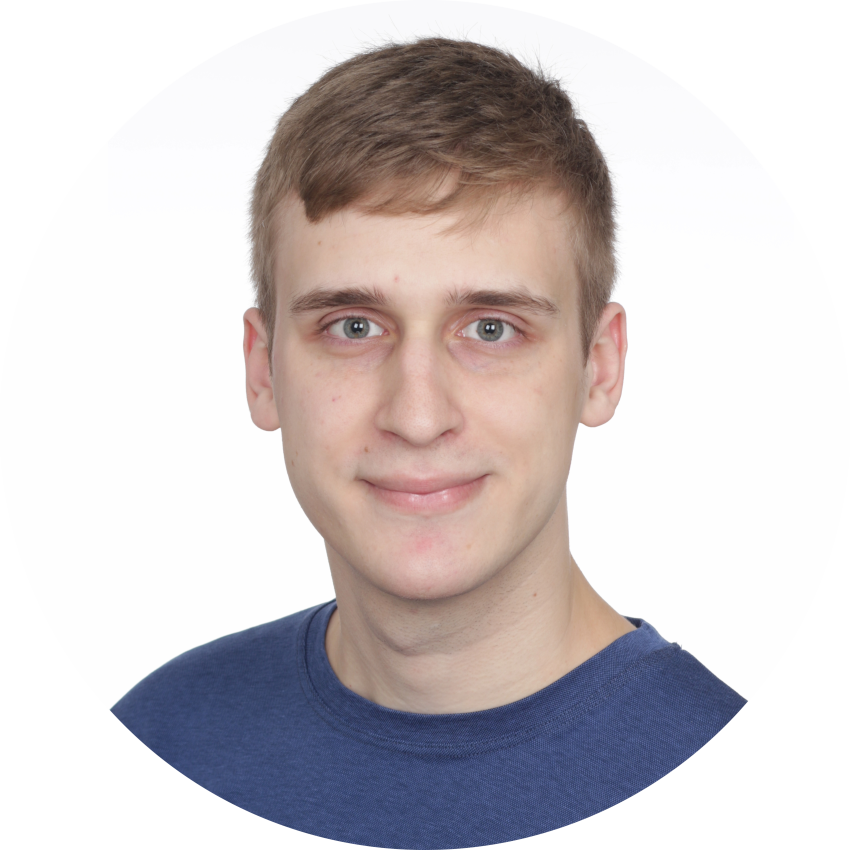
\includegraphics[width=50mm]{Photo_compressed_round.png}
    \end{minipage}
\end{tcolorbox}
\setstretch{1.1} % Spacing for the rest of the document

% ==================== Education ====================
\vspace{-2.5mm}
\begin{ItemizeSection}{Education}
    \item \PlaceAndTime{Computational Engineering (CE) M.Sc.}{04.2023 -- 12.2025} \\
    \textbf{(Specialization Computational Robotics)} \\
    TU Darmstadt (final grade \numprint{2.1}) \\
    Thesis (grade \numprint{1.7}):
    \begin{ItemizeSubsection}
        \item Topic: Adding spatial awareness to embedding-based anomaly detection methods for automated industrial inspection
        %\item Institute: Institute for Simulation, System optimisation and Robotics (SIM)
        \item Key outcomes: developed an anomaly detection method with 95\% accuracy by combining classical algorithms with foundation models (Python, PyTorch, Transformers)
    \end{ItemizeSubsection}

    \item \PlaceAndTime{Computational Engineering Science (CES) B.Sc.}{10.2018 -- 04.2023} \\
    RWTH Aachen University (final grade \numprint{2.4}) \\
    Thesis (grade \numprint{1.7}):
    \begin{ItemizeSubsection}
        \item Topic: Balancing a 2D inverted pendulum with a Franka Panda robotic arm
        %\item Institute: Institute for Data Science in Mechanical Engineering (DSME)
        \item Key outcomes: developed inverse kinematics, inverse dynamics, and control algorithms that enabled the robot to balance a 2-DOF inverse pendulum (ROS, C++, Python)
    \end{ItemizeSubsection}

    \item \PlaceAndTime{High school}{09.2017 -- 09.2018} \\
     Studienkolleg at Free University Berlin, technical course

    %\item \PlaceAndTime{Abitur}{09.2010 -- 05.2017} \\
    %Technical Lyceum of National Technical University of Ukraine \say{Kyiv Polytechnical Institute}
\end{ItemizeSection}

% ==================== Professional background ====================
\begin{ItemizeSection}{Professional experience}
    \item \PlaceAndTime{Student assistant at Goethe University Frankfurt}{06.2023 -- 07.2024} \\
    Buchmann Institute for Molecular Life Sciences (BMLS)
    \begin{ItemizeSubsection}
        \item Developed graphical slicing software with support of features unique to a bio-3D-printer (C\#, C++, Slic3r)
        \item Ported printer control software to a new hardware (C++, Arduino)
    \end{ItemizeSubsection}

    \item \PlaceAndTime{Intern at Continental AG}{03.2022 -- 05.2022}
    \begin{ItemizeSubsection}
        \item Developed a tool for generation of C code from CAN database (Python, C, CAPL)
        \item Automated software building process for a V850 microcontroller (CMake, Python)
    \end{ItemizeSubsection}

    \item \PlaceAndTime{Student assistant at RWTH Aachen University}{04.2021 -- 12.2021} \\
    Institute for Data Science in Mechanical Engineering (DSME)
    \begin{ItemizeSubsection}
        \item Implemented high-level APIs and developed control algorithms for a Franka Panda robotic arm (real-time Linux, C++, Python)
        \item Implemented a standalone (ROS-independent) software simulator for the robot (C++, Gazebo)
    \end{ItemizeSubsection}
\end{ItemizeSection}

\newpage
% ==================== Skills ====================
\begin{ItemizeSection}{IT skills}
    \item Software development:
    \begin{ItemizeSubsection}
        \item Expert: C, C++, Python, CMake
        \item Advanced: Matlab/Simulink, PyTorch, git, Linux, docker, \LaTeX
    \end{ItemizeSubsection}
    \item Hardware development:
    \begin{ItemizeSubsection}
        \item Expert: KiCAD, FreeCAD
        \item Basics: Autodesk Inventor
    \end{ItemizeSubsection}
    \item Embedded-development:
    \begin{ItemizeSubsection}
        \item Expert: C/C++ (Platforms: Atmel AVR, ARM, Raspberry Pi, Nvidia Jetson, x86\_64 real-time Linux), Python (Platforms: Nvidia Jetson, x86\_64 real-time Linux)
        \item Advanced: ROS, stationary robots (Franka Panda), mobile robots (Turtlebot, Jetbot)
        \item Basics: FPGA-Programming
    \end{ItemizeSubsection}
\end{ItemizeSection}


%\begin{ItemizeSection}{Akademic knowledge}
%    \item Expert: Data Structures and Algorithms
%    \item Advanced: Machine Learning (ML), Computer Vision (CV), \\ High-Performance Computing (HPC), Simulation technology (FEM, CFD), \\ Control theory, Robotics and navigation
%\end{ItemizeSection}

\begin{ItemizeSection}{Technical skills}
    \item Advanced: Soldering, PCB-Debugging
\end{ItemizeSection}

\begin{ItemizeSection}{Languages}
    \item Native: Ukrainian, Russian
    \item Fluent (C1): English, German
\end{ItemizeSection}

\begin{ItemizeSection}{Awards}
    \item Bronze medal at the International Physics Olympiad (IPhO), 2017
\end{ItemizeSection}

\end{document}
